\documentclass{article}
\usepackage[utf8]{inputenc}

\usepackage{geometry}
\usepackage[danish]{babel}
 \geometry{
 a4paper,
 total={140mm,227mm},
 left=35mm,
 top=35mm,
 }
 

\usepackage{float}
\usepackage{graphicx}
\usepackage{epstopdf}
\usepackage{amsmath}
\usepackage{amssymb}
\usepackage{mathtools} 
\usepackage{bm}
\usepackage{color}

\usepackage{hyperref}
\hypersetup{
    colorlinks=true,
    linkcolor=black,   
    urlcolor=black,
    filecolor=black,
} 
\urlstyle{same}

\usepackage{ dsfont }
\numberwithin{equation}{section}


%%%% tikz er pakken som gør det hele muligt %%%%
\usepackage[utf8]{luainputenc}
\usepackage{url}

\usepackage{tikz}
\usetikzlibrary{graphs,graphdrawing,quotes,babel} % vi har brug for nogle tikz-biblioteker
\usegdlibrary{trees, layered} % biblioteker til graf-placerings-algoritmer

%%%% et par kommandoer til at markere Όbne og lukkede grene %%%%

\newcommand{\closed}{child[white, level distance=5mm] {node[black] {$\times$}}}
\newcommand{\open}{child[white, level distance=5mm] {node[black] {$\bigcirc$}}}

%%%%% et par shortcuts for typesetting af de to sandhedsværdier %%%%%

\newcommand{\F}{\mathtt{F}}
\newcommand{\T}{\mathtt{T}}

%%%%%% navne på tableaureglerne: %%%%%%%%
%%  \tof er en forkortelse for "->F"
%% \lorf er en forkortelse for  "\/F"
%% \landf er en forkortelse for "/\F"
%% osv.


\newcommand{\lorf}{\ensuremath{\lor\F}}
\newcommand{\lort}{\ensuremath{\lor\T}}
\newcommand{\landf}{\ensuremath{\land\F}}
\newcommand{\landt}{\ensuremath{\land\T}}
\newcommand{\tof}{\ensuremath{\to\!\F}}
\newcommand{\tot}{\ensuremath{\to\!\T}}
\newcommand{\lrf}{\ensuremath{\leftrightarrow\!\F}}
\newcommand{\lrt}{\ensuremath{\leftrightarrow\!\T}}
\newcommand{\negf}{\ensuremath{\neg\F}}
\newcommand{\negt}{\ensuremath{\neg\T}}
\newcommand{\allf}{\ensuremath{\forall\F}}
\newcommand{\allt}{\ensuremath{\forall\T}}
\newcommand{\exf}{\ensuremath{\exists\F}}
\newcommand{\ext}{\ensuremath{\exists\T}}


%%%%%%% en kommando til at typesette formlerne i tableauer. Kommandoen kaldes med \formel{<nummer>}{<formel>}{<F hvis sættes falsk, T hvis sættes sand>} %%%%%%%%%%%%%%%%

\newcommand{\formel}[3]{{\color{red} \scriptsize #1} $#2: \ifx#3F \F \else \T \fi$}
 % sætter tikz op til at lave tableauer 

\title{01017 Diskret Matematik A2}
\author{s144107 Roar Nind Steffensen \\ s144063 Magnus Middelboe Søborg-Madsen}
\date{\today}

\begin{document}

\maketitle

\section*{Opgave A}

\begin{figure}[H]
    \centering
    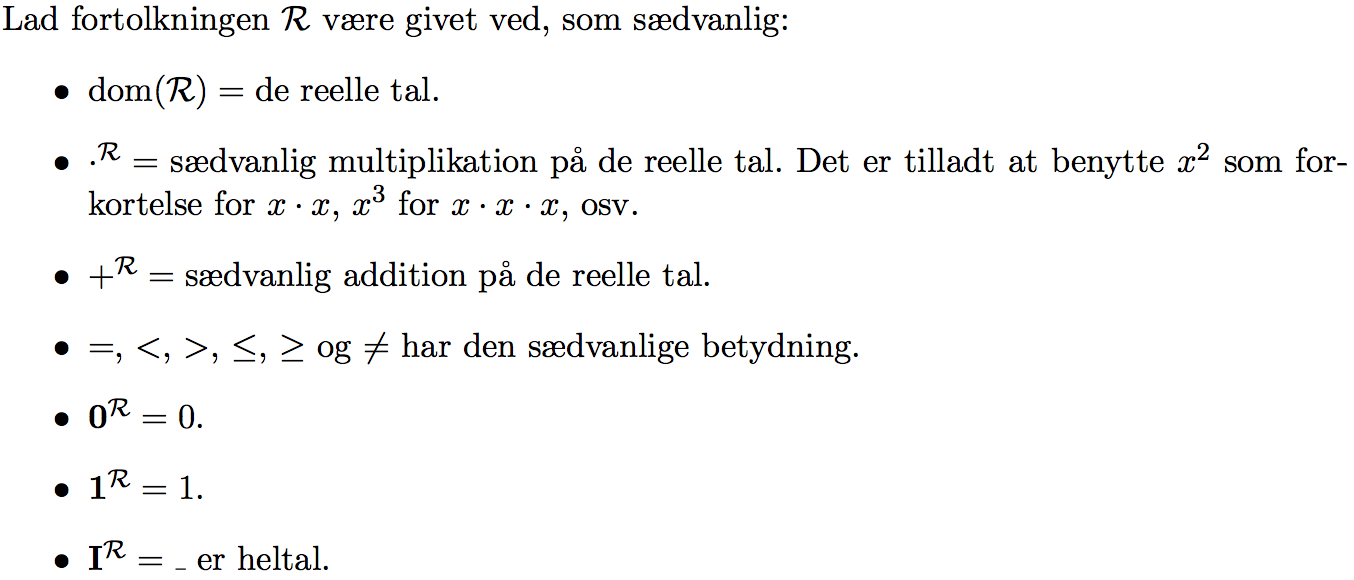
\includegraphics[width=1.0\textwidth]{opgA/opgA.png}
    \label{fig:opgA}
\end{figure}

Hver af følgende udsagn skrives med første-ordens prædikatslogik i fortolkningen $\mathcal{R}$. Når der optræder mere end ét reelt tal, bruger vi $x$ og $z$. $x$ er et vilkårligt reelt tal, $z$ er et reelt tal, vi giver egenskaben at være heltal med notationen $I(z)$. 

\begin{enumerate}
    \item Der findes et reelt tal som ikke er et heltal
    
        \begin{equation*}
            \exists x(\neg I(x))
        \end{equation*}
        
        \begin{flushright}
            Sandt, da ikke alle reelle tal er heltal, fx $\pi$ og $\frac{1}{2}$.
        \end{flushright} 
    
    \item Der findes et reelt tal som er større end alle heltal.
    
        \begin{equation*}
            \exists x \forall z \big(I(z) \rightarrow \left( x>z\right)\big)
        \end{equation*}
        
        \begin{flushright}
            Falskt, da der ingen øvre grænse er for heltal.
        \end{flushright} 
        
        
    \item Ethvert positivt heltal er kvadratet af et negativt reelt tal.
    
    Sætningen antages ækvivalent med: \\ "For alle positive heltal $z$, findes et negativt reelt tal $x$ der kvadreret giver $z$"
    
    \begin{equation*}
            \forall z \Big(\big((z>0) \wedge I(z)\big) \rightarrow \exists x\big((x<0) \wedge (x^2 = z)\big)\Big)
        \end{equation*}
        
        \begin{flushright}
            Sandt, da $\pm\sqrt{z} \in \mathbb{R}$ for $z \in \mathbb{Z}$, og kvadratet af et negativt reelt tal er positivt. Eksempel: heltallet 3 kan findes ved $(- \sqrt{3})^2$.
        \end{flushright} 
        
        
\end{enumerate}
\section*{Opgave B}

Efterfølgende udsagn testes mht. om de er \textit{gyldige} eller \textit{ikke gyldige}. Når vi skal vise, at et udsagn ikke er gyldigt, er det tilstrækkeligt at opstille en modmodel med en fortolkning, hvori udsagnet er falsk.\\ Når vi skal vise, at et udsagn er gyldigt, skal udsagnet vises at være sandt for en vilkårlig fortolkning.

\begin{enumerate}
    \item $\exists x P(x) \rightarrow \forall x P(x)$
    
    \begin{flushright}
        Ikke gyldig. \\ 
        Antag; $P(x)$: at være rig, og $x$: person. Én rig person, gør ikke alle rige (desværre).
    \end{flushright}
    
    %% SKRIV NOGET HER. SVARER TIL UGE 4, side 133.
    
    \item $\forall x (P(x) \vee \neg P(x))$
    
    \begin{flushright}
        Gyldig. \\ 
        Enten har $x$ egenskaben $P(x)$ ellers har $x$ ikke egenskaben $P(x)$.
    \end{flushright}

Uddybning til 2.: Lad $\mathcal{F}$ være en vilkårlig fortolkning. Vi giver $x$ en vilkårlig værdi $c$ i domænet af $\mathcal{F}$. Da $P(x)$ er sandt (hhv. falsk) for alle $x$, er $P(c)$ også sandt (hhv. falsk) for den vilkårlige værdi $c$.\\
\\
Case 1: $P(c)$ er sand. Så er $\neg P(c)$ falsk, og $P(c) \vee \neg P(c)$ er sandt. \\
Case 2: $P(c)$ er falsk. Så er $\neg P(c)$ sand, og $P(c) \vee \neg P(c)$ er sandt.\\
\\
Da udsagnet er $P(c) \vee \neg P(c)$ gyldigt for et vilkårligt valg af $c$ og for en vilkårlig fortolkning, er udsagnet $\forall x (P(x) \vee \neg P(x))$ gyldigt.

\end{enumerate}
\section*{Opgave C}

Følgende tre påstande tjekkes for gyldighed via tableau metoden.

\begin{enumerate}
    \item $ \forall x\big(P(x) \to Q(x)\big), \forall x P(x) \vDash  \forall x Q(x) $. \\
    

Vi husker dekompositionsreglerne for alkvantoren fra uge 5: Når vi substituerer $x$ i $\forall x A: \F$, skal vi indføre et nyt konstantsymbol. Når vi substituerer $x$ i $\forall x A: \T$, skal konstantsymbolet optræde tidligere på grenen. Vi håndterer derfor $\forall \F$ først.\\
\\
Hvis påstanden er skrevet op med præmisserne der medfører konklusionen får vi følgende tableau:


 \[
 \begin{tikzpicture}[align=center,every edge quotes/.style={magenta,auto,font=\scriptsize}]
   \graph[trie,tree layout,level sep=7mm,sibling distance=30mm] 
   {

     "\formel{1}{\Big(\forall x\big(P(x) \to Q(x)\big) \wedge \forall x P(x)\Big) \to \forall x Q(x)}{F}" 
     -- 

     "\formel{2}{\forall x\big(P(x) \to Q(x)\big) \wedge \forall x P(x)}{T} \\ 
     \formel{3}{\forall x Q(x)}{F}" 
     [> "$\tof$ på 1"] --  

    "\formel{4}{Q(c)}{F}"
    [> "$\allf$ på 3"] --

     "\formel{5}{\forall x\big(P(x) \to Q(x)\big)}{T} \\ 
     \formel{6}{\forall x P(x)}{T}" 
     [> "$\landt$ på 2"] -- 
    
    "\formel{7}{P(c) \to Q(c)}{T} \\ 
    \formel{8}{P(c)}{T}"
    [> "$\allt$ på 5 og 6"] --
    
    
    {
        "\formel{9}{P(c)}{F} \\ \times" --,
        "\formel{10}{Q(c)}{T} \\ \times" 
        [> "$\tot$ på 7"] --
    }
     
  };
  \end{tikzpicture}
\]

%% SKRIV NOGET HER OM ALKVANTOR OG SUBS. side 163.
Det kan dermed konkluderes, at påstanden er gyldig, da alle grene lukkes. \\
Dette kan også hurtigt ses fra påstanden selv; alle $x$ der har egenskaben $P(x)$ har også egenskaben $Q(x)$, samt information at alle $x$ \textbf{har} egenskaben $P(x)$, da må alle $x$ også have egenskaben $Q(x)$.\\
\\

\item $\forall x \big(P(x) \vee Q(x)\big) \vDash \forall x P(x) \vee \forall x Q(x)$. \\

Påstanden tjekkes med tableau metoden ligesom forrige opgave. Igen tager vi først trin, der indfører nye konstantsymboler.

 \[
 \begin{tikzpicture}[align=center,every edge quotes/.style={magenta,auto,font=\scriptsize}]
   \graph[trie,tree layout,level sep=7mm,sibling distance=30mm] 
   {

    "\formel{1}{\forall x \big(P(x) \vee Q(x)\big) \to \big(\forall x P(x) \vee \forall x Q(x) \big)}{F}" 
    -- 
     
    "\formel{2}{\forall x \big(P(x) \vee Q(x)\big)}{T} \\
    \formel{3}{\forall x P(x) \vee \forall x Q(x) }{F}"
    [> "$\tof$ på 1"] --  
    
    "\formel{4}{\forall x P(x)}{F} \\ 
    \formel{5}{\forall x Q(x)}{F}"
    [> "$\lorf$ på 3"] --  
     
    "\formel{6}{P(c_1)}{F} \\ 
    \formel{7}{Q(c_2)}{F}"
    [> "$\allf$ på 4 og 5"] --  
     
    "\formel{8}{P(c_1) \vee Q(c_1)}{T} \\
    \formel{9}{P(c_2) \vee Q(c_2)}{T}"
    [> "$\allt$ på 2"] --  
    

    
    {
        "\formel{10}{P(c_1)}{T} \\ \times" --,
        "\formel{11}{Q(c_1)}{T}" [> "$\lort$ på 8"] --
        {
          "\formel{12}{P(c_2)}{T} \\ \bigcirc",
          "\formel{13}{Q(c_2)}{T} \\ \times"  [> "$\lor\T$ på 9"]  -- 
        }
    }
  };
  \end{tikzpicture}
\]

Denne påstand er dermed ikke gyldig, da alle grene ikke kan lukkes. En mulig sandhedstildeling, der gør påstanden falsk, er $Q(c_1)$ og $P(c_2)$. \\
\\
Bonus: modmodel. Lad $x$ være studerende. $P(x)$ er piger, $Q(x)$ er drenge. Påstanden kan da læses: "Hvis alle studerende er enten drenge eller piger, er enten alle studerende drenge, eller alle studerende er piger." Påstanden er ikke gyldig.\\

\item $\exists x \forall y P(x,y) \vDash \forall y \exists x P(x,y)$. \\

Påstanden tjekkes med tableau metoden ligesom forrige opgaver.
Der indgår både dekomposition af alkvantor og eksistenskvantor. Vi tager først trin med $\forall \F$ og $\exists \T$ og indfører konstantstymboler. Derefter trin hvor vi substituerer de konstantsymboler, der optræder tidligere på grenen.

 \[
 \begin{tikzpicture}[align=center,every edge quotes/.style={magenta,auto,font=\scriptsize}]
   \graph[trie,tree layout,level sep=7mm,sibling distance=30mm] 
   {

    "\formel{1}{\exists x \forall y P(x,y) \to \forall y \exists x P(x,y)}{F}" 
    -- 
    
    "\formel{2}{\exists x \forall y P(x,y)}{T} \\ 
    \formel{3}{\forall y \exists x P(x,y)}{F}"
    [> "$\tof$ på 1"] -- 
    
    "\formel{4}{\forall y P(c_1,y)}{T}"
    [> "$\ext$ på 2"] -- 
    
    "\formel{5}{\exists x P(x,c_2)}{F}"
    [> "$\allf$ på 3"] -- 
    
    "\formel{6}{P(c_1,c_2)}{T}"
    [> "$\allt$ på 4"] -- 
    
    "\formel{7}{P(c_1,c_2)}{F} \\ \times"
    [> "$\exf$ på 5"] -- 

  };
  \end{tikzpicture}
\]

Grenen lukkes, så påstanden er gyldig. \\
\\
Eksempel på model: Lad $x$ være mænd, og $y$ kvinder. $P(x,y)$ betegner $x$ elsker $y$. Påstanden kan da læses: \\
\\
$\exists x \forall y P(x,y)$: Der findes en mand, der elsker alle kvinder. \\
$\forall y \exists x P(x,y)$: For hver kvinde findes en mand, der elsker hende.\\
$\exists x \forall y P(x,y) \vDash \forall y \exists x P(x,y)$: Hvis der findes en mand, der elsker alle kvinder, så kan der for hver kvinde findes en mand, der elsker hende.\\
\\
Påstanden er gyldig, da der i hvert fald findes én mand, der elsker alle kvinder.

\end{enumerate}
\section*{Opgave D}

\begin{enumerate}
    \item Hvordan tableau metoden kan anvendes til at afgøre om en formel i prædikatlogik er opfyldelig: \\
    
    %Hvis rodformlen i tableauet antages falsk, er formlen opfyldelig hvis én eller flere grene lukker. Hvis alle grene lukker er formlen tilmed gyldig. 
    Hvis rodformlen i tableauet antages sand, er formlen opfyldelig hvis én eller flere grene forbliver åbne. Hvis alle grene lukker, kan formlen ikke være sand; så er formlen en kontradiktion og dermed ikke opfyldelig.\\
    \\
    
    \item Historien om barberen:
    
    \begin{figure}[H]
        \centering
        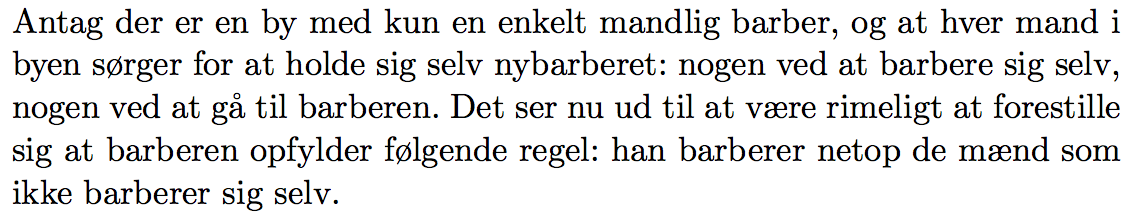
\includegraphics[width=0.8\textwidth]{opgD/barber.png}
        \label{fig:barber}
    \end{figure}
    
    Problemet med historien er; hvem barberer så barberen? \\
    Hvis barberen barberer sig selv, så må han ikke barbere sig selv; men hvis han ikke barberer sig selv, så barberer han sig selv.\\
    \\
    
    \item Analyse af barber problemet:
    
    Under den givne fortolkning $\mathcal{F}$ givet ved:
    
    \begin{figure}[H]
        \hspace{7 mm}
        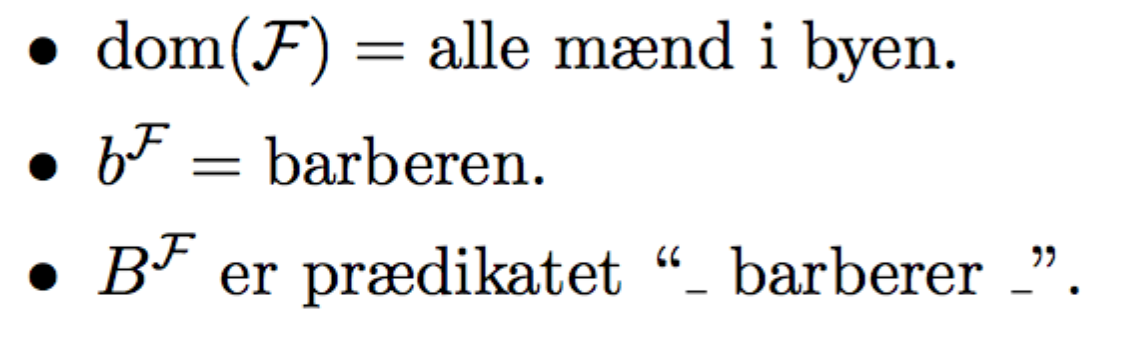
\includegraphics[width=0.4\textwidth]{opgD/barbFort.png}
        \label{fig:barbFort}
    \end{figure}
    
    Problemet bliver stilt op med med prædikationslogik som:
    
    \begin{equation*}
        \forall x (\neg B(x,x) \leftrightarrow B(b,x))
    \end{equation*}
    Udsagnet forstås som: "Barberen barberer dig, hvis og kun hvis du ikke barberer dig selv". Dette udsagns gyldighed kan kort tjekkes med tableau metoden:
    
     \[
 \begin{tikzpicture}[align=center,every edge quotes/.style={magenta,auto,font=\scriptsize}]
   \graph[trie,tree layout,level sep=7mm,sibling distance=30mm] 
   {

    "\formel{1}{\forall x (\neg B(x,x) \leftrightarrow B(b,x))}{T}" 
    -- 
    
    "\formel{2}{\neg B(b,b) \leftrightarrow B(b,b)}{T}"
    [> "$\allt$ på 1"] -- 
    
    {
        "\formel{3}{\neg B(b,b)}{T}\\
        \formel{4}{B(b,b)}{T}" -- "\formel{7}{B(b,b)}{F} \\ \times" [>"$\negt$ på 3"] ,
         "\formel{5}{\neg B(b,b)}{F}\\
        \formel{6}{B(b,b)}{F}" [>"$\leftrightarrow\T$ på 2"] -- "\formel{8}{B(b,b)}{T}  \\ \times" [>"$\negf$ på 5"]
    }
    
  };
  \end{tikzpicture}
\]

Alle grene bliver lukket. Udsagnet er derfor ikke opfyldeligt og dermed ikke gyldigt.
\end{enumerate}
\section*{Opgave E}

\begin{enumerate}
    \item $A=\{x \in \mathbb{R} | x^2 - 3x = 4 \}$.\\
    Mængden A indeholder alle reelle løsninger til ligningen $x^2-3x=4$ dvs.: $A = \{-1,4\}$.
    
    \item $B=\{x\in \mathbb{Z}|-3 \leq x < 3\}$. \\
    Mængden B indeholder alle heltal fra $-$3 inklusiv til
3 eksklusiv, dvs.: $B=\{-3, -2, -1, 0, 1, 2\}$.

    \item $C = \{ x \in \mathbb{Z} | -3 \leq x < 3 \wedge x^2-3x=4 \}$. \\
    Mængden C er lig med $A \cap B$ dvs.: $C = \{ -1 \}$.
    
    \item $D = \{ x \in \mathbb{Z} | -3 \leq x < 3 \wedge x^2-3x \neq 4 \}$ \\
    Mængden D er lig med $B \-- A$, elementerne i $B$, bortset løsningerne til ligningen $x^2-3x=4$, dvs. $D = \{ -3, -2, 0, 1, 2 \}$. \\
    \\
    
    Det faktum at $C$ og $D$ kan beskrives ud fra $A$ og $B$, ses ud fra mængdekriterierne. Vi anvender definitionerne af foreningsmængde og mængdedifferens. \\
    Elementerne i $C$ overholder kriteriet for at tilhøre $B$ og kriteriet for at tilhøre $A$. Dette er netop kriteriet for at tilhøre fællesmængden $A \cap B$.\\ Elementerne i $D$ opfylder kriteriet for at tilhøre $B$, men opfylder netop ikke kriteriet for at tilhøre $A$. Det er netop kriteriet for at tilhøre mængdedifferensen $B \-- A$.
    
\end{enumerate}
\section*{Opgave F}

Følgende tre ligheder eftervises:

\begin{enumerate}
    \item $A \cup (B \cap C) = (A \cup B) \cap (A \cup C)$.\\
    
    Ved at skrive lighederne om til udsagnslogik, får vi: 
    \begin{equation*}
        A \vee (B \wedge C) \equiv (A \vee B) \wedge (A \vee C)
    \end{equation*}
    
    Ved at se på logiske ækvivalenser ser vi at dette præcis er reglen for distributivitet af $\wedge$ over $\vee$, givet fra slides i selvstudium:
    
    \begin{figure}[H]
        \centering
        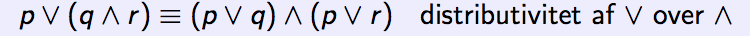
\includegraphics[width=0.7\textwidth]{opgF/WoverV.png}
        \label{fig:WoverV}
    \end{figure}
    
    Lighed 1 er dermed bevist.\\
    \\
    
    \item $A \-- (A \cap B) = A \-- B$. \\
    
    Ved at skrive lighederne om til udsagnslogik, får vi: 
    \begin{equation*}
        A \wedge \neg (A \wedge B) \equiv A \wedge \neg B
    \end{equation*}
    
    Ved at bruge De Morgan-loven: 
    
    \begin{figure}[H]
        \centering
        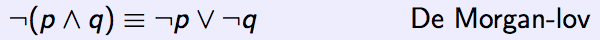
\includegraphics[width = 0.5\textwidth]{opgF/DML1.png}
        \label{fig:DML1}
    \end{figure}
    
    Får vi venstresiden til:
    \begin{equation*}
        A \wedge \neg (A \wedge B) \equiv A \wedge (\neg A \vee \neg B) )
    \end{equation*}
    For at have alle mellemregninger med, bruger vi nu reglen for distributivitet af $\wedge$ over $\vee$:
    
    \begin{figure}[H]
        \centering
        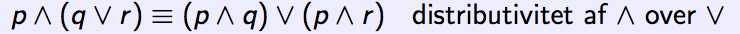
\includegraphics[width=0.7\textwidth]{opgF/VoverW.png}
        \label{fig:VoverW}
    \end{figure}
    
    Dermed får vi: 
    
    \begin{equation*}
        A \wedge (\neg A \vee \neg B) ) \equiv (A \wedge \neg A) \vee (A \wedge \neg B)
    \end{equation*}
    
    Eftersom $A \wedge \neg A$ er en kontradiktion, bliver venstresiden da ækvivalent med:
    
    \begin{equation*}
        (A \wedge \neg A) \vee (A \wedge \neg B) \equiv A \wedge \neg B
    \end{equation*}
    
    Lighed 2 er dermed bevist.\\
    I denne opgave fås en klar forståelse for hvordan mængdedifferensen $A-B$ skal forstås, når $B$ ikke er indeholdt i $A$: Behold elementerne i $A$, fjern elementerne i foreningsmængden.
    
    \item $A \cap ( A \cup B) = A$.

    \textbf{Metode 1}. For at vise at mængdelighed skal vi vise at mængderne er delmængder er hinanden. Dvs. skal vi vise \textbf{3a.} $A \subseteq A \cap ( A \cup B)$ og \textbf{3b.} $A \cap ( A \cup B) \subseteq A$.\\
    \\
    \textbf{3a.} $A \subseteq A \cap ( A \cup B)$ \\
    Betragt et vilkårligt $x$ i $A$: $x \in A$. Så tilhører $x$ også foreningsmængden: $x \in A \cup B$. Da $x$ både tilhører $A$ og $A \cup B$, tilhører $x$ fællesmængden:  $x \in A \cap ( A \cup B)$. Da ovenstående gælder for alle $x$ i $A$, er $A \subseteq A \cap ( A \cup B)$.\\
    \\
    \textbf{3b.} $A \cap ( A \cup B) \subseteq A$\\
    Betragt et vilkårligt $x$ i fællesmængden $A \cap ( A \cup B)$: $x \in A \cap ( A \cup B)$. Da $x$ tilhører fællesmængden, tilhører $x$ både $A$ og $A \cup B$. Dvs. $x \in A$. Da ovenstående gælder for alle $x$ i $A \cap ( A \cup B)$, er $A \cap ( A \cup B) \subseteq A$.\\
    
    \textbf{Metode 2}. Vi oversætter mængdeligheden til udsagnslogik og tjekker med en sandhedstabel. $A \cap ( A \cup B) = A$ oversættes til $A \land (A \lor B) \leftrightarrow A$.
    
    \begin{table}[H]
\centering
\begin{tabular}{c|c|c|c|c}
$A$ & $B$ & $(A \lor B)$ & $A \land (A \lor B)$ & $ A \land (A \lor B) \leftrightarrow A$ \\ \hline
F & F & F & F & T \\
F & T & T & F & T \\
T & F & T & T & T \\
T & T & T & T & T \\
\end{tabular}
\end{table}
    
Det ses at udsagnet $A \land (A \lor B) \leftrightarrow A$ er gyldigt, så $A \cap ( A \cup B) = A$.
    
    % Sprogligt bevis: Antag at $x \in A \cap (A \cup B)$. Da $A \in A \cup B$, da må $x \in A$. Altså må $A \cap (A \cup B) = A$.
    
\end{enumerate}

\begin{figure}[H]
    \centering
    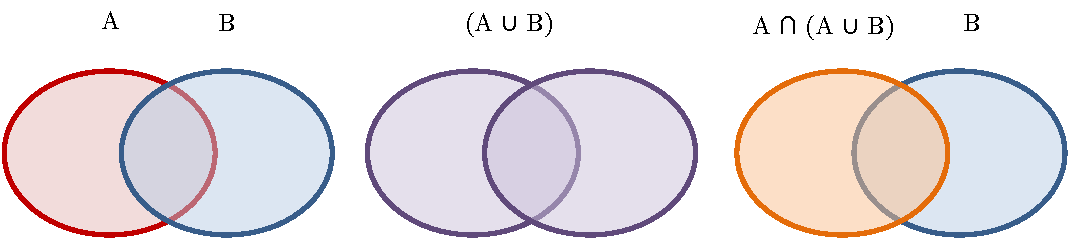
\includegraphics[width=1.0\textwidth]{opgF/F3.pdf}
    \caption{Betragt mængderne  \textcolor{red}{$A$} og \textcolor{blue}{$B$}, og deres foreningsmængde \textcolor{purple}{$A \cup B$}. Alle elementer, der tilhører fællesmængden \textcolor{orange}{$A \cap ( A \cup B)$}, tilhører \textcolor{red}{$A$} (og vice versa).}
    \label{fig:F3}
\end{figure}





\end{document}
